\documentclass[aspectratio=169,professionalfonts]{beamer}

\usetheme{AnnArbor}
\usecolortheme{dolphin}
\setbeamertemplate{navigation symbols}{}
\setbeamertemplate{footline}[frame number]

\usepackage{fontspec}
\setsansfont{Noto Sans}
\setmonofont{Noto Sans Mono}
\usepackage{booktabs}
\usepackage{array}
\usepackage{tabularx}
\usepackage{tikz}
\usetikzlibrary{positioning,arrows.meta,shapes.geometric}
\usepackage{listings}
\usepackage{xcolor}

\definecolor{sqlbg}{RGB}{248,248,248}
\definecolor{sqlkw}{RGB}{20,70,150}
\definecolor{sqlcm}{RGB}{90,90,90}
\definecolor{accent}{RGB}{0,89,156}

\lstdefinestyle{sqlstyle}{
  language=SQL,
  basicstyle=\ttfamily\scriptsize,
  keywordstyle=\color{sqlkw}\bfseries,
  commentstyle=\color{sqlcm},
  backgroundcolor=\color{sqlbg},
  frame=single,
  rulecolor=\color{black!20},
  columns=fullflexible,
  keepspaces=true,
  showstringspaces=false,
  breaklines=true,
  xleftmargin=0.5em,
  xrightmargin=0.5em,
  aboveskip=0.4em,
  belowskip=0.2em
}

\newcommand{\code}[1]{\texttt{#1}}
\newcommand{\smallnote}[1]{\vspace{0.3em}{\scriptsize\color{black!65}#1}}

\title[MySQL classicmodels]{MySQL Sample Database: \code{classicmodels}}
\subtitle{Tutorial nhập môn cơ sở dữ liệu mẫu trong MySQL}
\author{DSAI1002 -- Database Practice}
\institute{Faculty of Data Science \& Artificial Intelligence}
\date{2026}

\begin{document}

\begin{frame}
  \titlepage
  \smallnote{Nguồn nội dung: MySQL Tutorial -- MySQL Sample Database.}
\end{frame}

\section{Giới thiệu}

\begin{frame}{Mục tiêu bài học}
Sau bài học này, người học có thể:
\begin{enumerate}
  \item Hiểu \code{classicmodels} là gì và vì sao thường dùng khi học MySQL.
  \item Nhận diện các nhóm dữ liệu chính trong database.
  \item Hiểu vai trò của các bảng quan trọng trong schema.
  \item Đọc sơ đồ ERD để theo dõi quan hệ giữa các bảng.
  \item Chuẩn bị database mẫu để thực hành các bài MySQL tiếp theo.
\end{enumerate}
\end{frame}

\begin{frame}{\code{classicmodels} database là gì?}
\begin{block}{Ý tưởng chính}
\code{classicmodels} là cơ sở dữ liệu mẫu mô phỏng một doanh nghiệp bán lẻ các mô hình xe cổ thu nhỏ.
\end{block}
\vspace{0.4em}
Database này chứa dữ liệu nghiệp vụ gần với hệ thống kinh doanh thực tế, phù hợp để luyện truy vấn SQL từ cơ bản đến nâng cao.
\end{frame}

\begin{frame}{Các nhóm dữ liệu trong \code{classicmodels}}
\begin{columns}[T,onlytextwidth]
\column{0.48\textwidth}
\begin{itemize}
  \item Khách hàng
  \item Sản phẩm
  \item Dòng sản phẩm
  \item Đơn hàng bán
  \item Chi tiết đơn hàng
\end{itemize}
\column{0.48\textwidth}
\begin{itemize}
  \item Thanh toán của khách hàng
  \item Nhân viên
  \item Văn phòng bán hàng
  \item Cấu trúc báo cáo nhân sự
\end{itemize}
\end{columns}
\end{frame}

\begin{frame}{Vì sao nên dùng \code{classicmodels}?}
\begin{enumerate}
  \item Dữ liệu thực tế hơn các ví dụ quá nhỏ chỉ có một hoặc hai bảng.
  \item Phù hợp để luyện \code{SELECT}, \code{WHERE}, \code{ORDER BY}, \code{GROUP BY}, \code{JOIN}, subquery, view và stored procedure.
  \item Có quan hệ khóa chính - khóa ngoại giữa nhiều bảng.
  \item Dễ đặt câu hỏi phân tích kinh doanh: khách hàng mua nhiều nhất, sản phẩm bán chạy, doanh thu theo quốc gia, đơn hàng chưa thanh toán.
\end{enumerate}
\end{frame}

\section{Cài đặt database mẫu}

\begin{frame}{Tải database mẫu}
\begin{itemize}
  \item Tải file mẫu từ trang MySQL Tutorial.
  \item File thường ở dạng nén:
\end{itemize}
\begin{center}
\fbox{\Large\code{sampledatabase.zip}}
\end{center}
\begin{itemize}
  \item Sau khi tải, cần giải nén để lấy file SQL dùng để import vào MySQL Server.
\end{itemize}
\end{frame}

\begin{frame}{Giải nén file database mẫu}
\begin{itemize}
  \item Có thể dùng công cụ giải nén như \code{7-Zip}.
  \item Sau khi giải nén, thường nhận được file:
\end{itemize}
\begin{center}
\fbox{\Large\code{mysqlsampledatabase.sql}}
\end{center}
\begin{block}{File SQL chứa gì?}
Các câu lệnh để tạo database, tạo bảng và thêm dữ liệu mẫu vào bảng.
\end{block}
\end{frame}

\begin{frame}{Hai cách import vào MySQL Server}
\begin{columns}[T,onlytextwidth]
\column{0.48\textwidth}
\begin{block}{Cách 1}
Dùng \code{mysql command-line client}
\end{block}
\begin{itemize}
  \item Nhanh
  \item Phù hợp khi đã quen terminal
\end{itemize}
\column{0.48\textwidth}
\begin{block}{Cách 2}
Dùng \code{MySQL Workbench}
\end{block}
\begin{itemize}
  \item Trực quan
  \item Phù hợp với người mới học
\end{itemize}
\end{columns}
\end{frame}

\begin{frame}[fragile]{Cách 1: Import bằng command line}
Giả sử file SQL nằm trong thư mục \code{Downloads}:
\begin{lstlisting}[style=sqlstyle,language=bash]
mysql -u root -p < "C:\Users\YourName\Downloads\mysqlsampledatabase.sql"
\end{lstlisting}
\begin{itemize}
  \item \code{-u root}: đăng nhập bằng user \code{root}.
  \item \code{-p}: yêu cầu nhập mật khẩu.
  \item \code{<}: chuyển nội dung file SQL vào MySQL để thực thi.
\end{itemize}
\end{frame}

\begin{frame}{Cách 2: Import bằng MySQL Workbench}
\begin{enumerate}
  \item Mở MySQL Workbench và kết nối tới MySQL Server.
  \item Vào menu \code{Server > Data Import}.
  \item Chọn file \code{mysqlsampledatabase.sql}.
  \item Nhấn \code{Start Import}.
  \item Kiểm tra schema \code{classicmodels} xuất hiện trong danh sách.
\end{enumerate}
\end{frame}

\begin{frame}[fragile]{Kiểm tra sau khi import}
\begin{lstlisting}[style=sqlstyle]
SHOW DATABASES;
USE classicmodels;
SHOW TABLES;
\end{lstlisting}
\vspace{0.4em}
Nếu import thành công, danh sách bảng sẽ gồm các bảng như \code{customers}, \code{employees}, \code{offices}, \code{orders}, \code{orderdetails}, \code{payments}, \code{productlines}, \code{products}.
\end{frame}

\section{Schema và ERD}

\begin{frame}{Các bảng chính trong schema}
\small
\begin{tabularx}{\textwidth}{>{\ttfamily}l X}
\toprule
Bảng & Ý nghĩa \\
\midrule
customers & Lưu dữ liệu khách hàng \\
products & Lưu danh sách các mô hình xe cổ \\
productlines & Lưu các dòng sản phẩm \\
orders & Lưu các đơn hàng bán \\
orderdetails & Lưu chi tiết từng dòng sản phẩm trong mỗi đơn hàng \\
payments & Lưu các khoản thanh toán của khách hàng \\
employees & Lưu thông tin nhân viên và cấu trúc báo cáo \\
offices & Lưu dữ liệu văn phòng bán hàng \\
\bottomrule
\end{tabularx}
\end{frame}

\begin{frame}{ER Diagram: quan hệ tổng quát}
\centering
\resizebox{0.84\textwidth}{!}{%
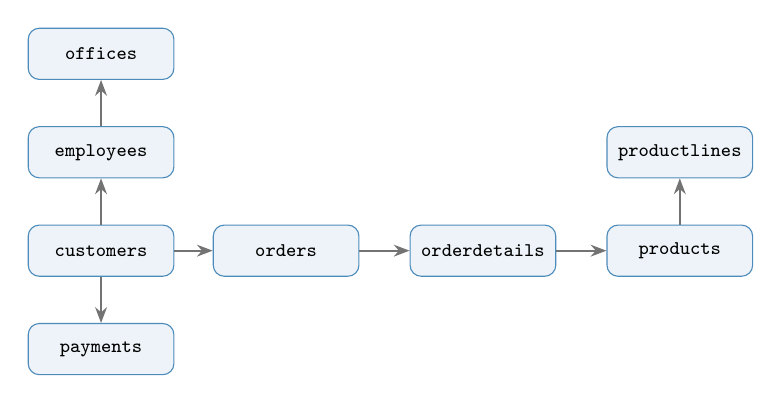
\begin{tikzpicture}[
  tbl/.style={rectangle, rounded corners, draw=accent!70, fill=accent!7, minimum width=1.85cm, minimum height=0.65cm, font=\scriptsize\ttfamily, align=center},
  rel/.style={-{Stealth[length=2mm]}, thick, draw=black!55}
]
\node[tbl] (customers) at (0,0) {customers};
\node[tbl] (orders) at (2.35,0) {orders};
\node[tbl] (orderdetails) at (4.85,0) {orderdetails};
\node[tbl] (products) at (7.35,0) {products};
\node[tbl] (productlines) at (7.35,1.25) {productlines};
\node[tbl] (payments) at (0,-1.25) {payments};
\node[tbl] (employees) at (0,1.25) {employees};
\node[tbl] (offices) at (0,2.50) {offices};

\draw[rel] (customers) -- (orders);
\draw[rel] (orders) -- (orderdetails);
\draw[rel] (orderdetails) -- (products);
\draw[rel] (products) -- (productlines);
\draw[rel] (customers) -- (payments);
\draw[rel] (customers) -- (employees);
\draw[rel] (employees) -- (offices);
\end{tikzpicture}%
}
\smallnote{Sơ đồ rút gọn; bảng \code{employees} còn có quan hệ tự tham chiếu \code{reportsTo}.}
\end{frame}

\begin{frame}{Nhóm bảng về khách hàng và sản phẩm}
\footnotesize
\begin{block}{\code{customers}}
Mã khách hàng, tên khách hàng, liên hệ, địa chỉ, quốc gia, nhân viên phụ trách, hạn mức tín dụng.
\end{block}
\vspace{0.45em}
\begin{block}{\code{products}}
Mã sản phẩm, tên sản phẩm, dòng sản phẩm, nhà cung cấp, tồn kho, giá mua, giá bán đề xuất.
\end{block}
\vspace{0.45em}
\begin{block}{\code{productlines}}
Phân loại sản phẩm: Classic Cars, Motorcycles, Planes, Ships, Trains, Vintage Cars, v.v.
\end{block}
\end{frame}

\begin{frame}{Nhóm bảng về đơn hàng và thanh toán}
\footnotesize
\begin{block}{\code{orders}}
Mã đơn hàng, ngày đặt, ngày yêu cầu giao, ngày giao thực tế, trạng thái, mã khách hàng.
\end{block}
\vspace{0.45em}
\begin{block}{\code{orderdetails}}
Mã đơn hàng, mã sản phẩm, số lượng đặt, giá bán từng sản phẩm, thứ tự dòng hàng.
\end{block}
\vspace{0.45em}
\begin{block}{\code{payments}}
Mã khách hàng, mã giao dịch, ngày thanh toán và số tiền thanh toán.
\end{block}
\end{frame}

\begin{frame}{Nhóm bảng về nhân sự và văn phòng}
\begin{columns}[T,onlytextwidth]
\column{0.48\textwidth}
\begin{block}{\code{employees}}
Lưu mã nhân viên, họ tên, email, chức danh, văn phòng làm việc và người quản lý trực tiếp.
\end{block}
\column{0.48\textwidth}
\begin{block}{\code{offices}}
Lưu mã văn phòng, thành phố, số điện thoại, địa chỉ, quốc gia và khu vực.
\end{block}
\end{columns}
\vspace{0.5em}
\begin{alertblock}{Lưu ý}
Bảng \code{employees} có quan hệ tự tham chiếu để biểu diễn cấu trúc báo cáo trong tổ chức.
\end{alertblock}
\end{frame}

\section{Truy vấn mẫu}

\begin{frame}[fragile]{Truy vấn kiểm tra nhanh}
\begin{lstlisting}[style=sqlstyle]
USE classicmodels;

SHOW TABLES;

SELECT customerNumber, customerName, country
FROM customers
LIMIT 10;
\end{lstlisting}
\end{frame}

\begin{frame}[fragile]{Xem sản phẩm và đơn hàng gần đây}
\begin{lstlisting}[style=sqlstyle]
SELECT productCode, productName, productLine, buyPrice, MSRP
FROM products
LIMIT 10;

SELECT orderNumber, orderDate, status, customerNumber
FROM orders
ORDER BY orderDate DESC
LIMIT 10;
\end{lstlisting}
\end{frame}

\begin{frame}[fragile]{Tính doanh thu từng dòng đơn hàng}
\begin{lstlisting}[style=sqlstyle]
SELECT orderNumber,
       productCode,
       quantityOrdered,
       priceEach,
       quantityOrdered * priceEach AS lineRevenue
FROM orderdetails
LIMIT 10;
\end{lstlisting}
\begin{block}{Ý nghĩa}
Mỗi dòng trong \code{orderdetails} biểu diễn một sản phẩm trong một đơn hàng. Doanh thu dòng hàng được tính bằng số lượng nhân với đơn giá.
\end{block}
\end{frame}

\begin{frame}[fragile]{JOIN: lấy đơn hàng kèm tên khách hàng}
\begin{lstlisting}[style=sqlstyle]
SELECT o.orderNumber,
       o.orderDate,
       o.status,
       c.customerName
FROM orders o
JOIN customers c
  ON o.customerNumber = c.customerNumber
LIMIT 10;
\end{lstlisting}
\smallnote{Khóa \code{customerNumber} giúp kết nối \code{orders} với \code{customers}.}
\end{frame}

\begin{frame}[fragile]{JOIN: lấy sản phẩm kèm dòng sản phẩm}
\begin{lstlisting}[style=sqlstyle]
SELECT p.productCode,
       p.productName,
       p.productLine,
       pl.textDescription
FROM products p
JOIN productlines pl
  ON p.productLine = pl.productLine
LIMIT 10;
\end{lstlisting}
\smallnote{Truy vấn này giúp biết mỗi sản phẩm thuộc dòng sản phẩm nào.}
\end{frame}

\begin{frame}[fragile]{GROUP BY: tính doanh thu theo đơn hàng}
\begin{lstlisting}[style=sqlstyle]
SELECT od.orderNumber,
       SUM(od.quantityOrdered * od.priceEach) AS totalRevenue
FROM orderdetails od
GROUP BY od.orderNumber
ORDER BY totalRevenue DESC
LIMIT 10;
\end{lstlisting}
\begin{block}{Mẫu tư duy}
Chọn khóa nhóm $\rightarrow$ tính chỉ tiêu tổng hợp $\rightarrow$ sắp xếp kết quả.
\end{block}
\end{frame}

\begin{frame}{Các chủ đề MySQL có thể học}
\small
\begin{tabularx}{\textwidth}{>{\bfseries}l X}
\toprule
Chủ đề & Ví dụ thực hành \\
\midrule
Basic SELECT & Lấy danh sách khách hàng, sản phẩm \\
WHERE & Lọc khách hàng theo quốc gia \\
ORDER BY & Sắp xếp đơn hàng theo ngày \\
GROUP BY & Tính doanh thu theo khách hàng hoặc đơn hàng \\
JOIN & Kết hợp khách hàng với đơn hàng \\
Subquery & Tìm khách hàng có doanh thu cao hơn trung bình \\
View / Procedure & Tạo báo cáo và thủ tục thống kê \\
Index & Tối ưu truy vấn theo khóa \\
\bottomrule
\end{tabularx}
\end{frame}

\section{Thực hành và ôn tập}

\begin{frame}{Bài tập 1: Import database}
\begin{block}{Yêu cầu}
Import database \code{classicmodels} vào MySQL Server.
\end{block}
Sau đó kiểm tra bằng các lệnh:
\begin{itemize}
  \item \code{SHOW DATABASES;}
  \item \code{USE classicmodels;}
  \item \code{SHOW TABLES;}
\end{itemize}
\end{frame}

\begin{frame}[fragile]{Bài tập 2: Truy vấn 10 khách hàng đầu tiên}
Hiển thị \code{customerNumber}, \code{customerName}, \code{city}, \code{country}.
\begin{lstlisting}[style=sqlstyle]
SELECT customerNumber, customerName, city, country
FROM customers
LIMIT 10;
\end{lstlisting}
\end{frame}

\begin{frame}{Bài tập 3--4: Sản phẩm và doanh thu}
\begin{block}{Bài tập 3}
Truy vấn danh sách sản phẩm thuộc dòng sản phẩm \code{Classic Cars}. Hiển thị \code{productCode}, \code{productName}, \code{productLine}, \code{MSRP}.
\end{block}
\begin{block}{Bài tập 4}
Tính tổng doanh thu từng đơn hàng từ bảng \code{orderdetails}, dùng công thức \code{quantityOrdered * priceEach}, sau đó nhóm theo \code{orderNumber}.
\end{block}
\end{frame}

\begin{frame}{Bài tập 5: JOIN đơn hàng và khách hàng}
Viết truy vấn JOIN để hiển thị đơn hàng kèm tên khách hàng.
\vspace{0.5em}
\begin{itemize}
  \item Bảng 1: \code{orders}
  \item Bảng 2: \code{customers}
  \item Trường kết nối: \code{customerNumber}
\end{itemize}
\end{frame}

\begin{frame}{Câu hỏi tự luận}
\begin{enumerate}
  \item \code{classicmodels} database mô phỏng nghiệp vụ gì?
  \item Vì sao \code{classicmodels} phù hợp để học MySQL?
  \item Bảng \code{orderdetails} có vai trò gì?
  \item Vì sao cần bảng \code{productlines} nếu đã có bảng \code{products}?
  \item ER Diagram giúp ích gì khi học database \code{classicmodels}?
\end{enumerate}
\end{frame}

\begin{frame}{Câu hỏi trắc nghiệm}
\small
\begin{enumerate}
  \item \code{classicmodels} mô phỏng lĩnh vực nào?\newline
  A. Bán lẻ mô hình xe cổ thu nhỏ \quad B. Quản lý bệnh viện \quad C. Thư viện số \quad D. Mạng xã hội
  \item Bảng nào lưu dữ liệu khách hàng?\newline
  A. \code{products} \quad B. \code{customers} \quad C. \code{orders} \quad D. \code{offices}
  \item Bảng nào lưu chi tiết dòng sản phẩm trong đơn hàng?\newline
  A. \code{payments} \quad B. \code{employees} \quad C. \code{orderdetails} \quad D. \code{productlines}
  \item Bảng nào lưu dữ liệu thanh toán?\newline
  A. \code{products} \quad B. \code{orders} \quad C. \code{offices} \quad D. \code{payments}
\end{enumerate}
\end{frame}

\begin{frame}{Tóm tắt bài học}
\begin{itemize}
  \item \code{classicmodels} là database mẫu trong MySQL, mô phỏng doanh nghiệp bán mô hình xe cổ thu nhỏ.
  \item Schema gồm \code{customers}, \code{products}, \code{productlines}, \code{orders}, \code{orderdetails}, \code{payments}, \code{employees}, \code{offices}.
  \item Database này phù hợp để luyện \code{SELECT}, \code{JOIN}, \code{GROUP BY}, truy vấn tổng hợp, view và stored procedure.
  \item ER Diagram giúp người học hiểu quan hệ giữa các bảng trước khi viết truy vấn.
\end{itemize}
\end{frame}

\begin{frame}{Từ khóa chính}
\centering
\Large
\code{MySQL} \quad \code{classicmodels} \quad \code{Schema} \\
\vspace{0.5em}
\code{ER Diagram} \quad \code{SELECT} \quad \code{JOIN} \\
\vspace{0.5em}
\code{GROUP BY} \quad \code{View} \quad \code{Stored Procedure}
\end{frame}

\end{document}
